Python\footnote{We use `Python' to refer to CPython, the popular C language implementation of Python, which is dominant in computational science.}\footnote{This section is adapted from a paper recently submitted to Computing in Science and Engineering \cite{kailasa2022pyexafmm}} fulfills many of the key usability criteria for scientific software. Cross platform builds are trivial with open source build systems such as Conda, and its simple syntax and large scientific computing ecosystem of numerical libraries allows for rapid dissemination amongst the wider community. Its simplicity allows Computational Scientists to spend more time exploring their science, and less time being confused by software quirks, memory errors, and the nightmare of incompatible dependencies, which conspire to drain productivity in lower level languages.

With this in mind we sought to assess the suitability of Python as a base language for fast algorithm software. With stable MPI bindings for multi-node development \cite{dalcin2021mpi4py}, Python's major pitfall is its restriction to run in a single thread due a software construction called the `Global Interpreter Lock' (GIL). Libraries for high performance computational science have traditionally bypassed the issue of the GIL by using Python's C interface to call extensions built in C or other compiled languages which can be multithreaded or compiled to target special hardware features, thus enabling hierarchical parallelism.

Recently `just in time' (JIT), compilers have emerged as a technique for compiling high-level languages to fast machine code. The idea being that a user is able to rapidly iterate on their algorithm, with the compiler taking responsibility to deliver performance. The Numba compiler For Python was written to targets and optimise code written with NumPy's $n$-dimensional array, or `ndarray', data structure, which are homogenously typed containers stored contiguously in memory \cite{lam2015numba}. Its power comes from the ability to generate multithreaded architecture optimised compiled code while \textit{only writing Python}. The promise of Numba is the ability to develop applications with speed that can rival C++ or Fortran, while retaining the simplicity and productivity of working in Python. We tested Numba's suitability by developing `PyExaFMM', an implementation of the three-dimensional Kernel Independent FMM \cite{kailasa2022pyexafmm}.

\subsection*{Numba}

Numba is a compiler built with LLVM, a framework for building custom compilers, to target a subset of Python code that uses ndarrays. LLVM provides an API for generating machine code for different hardware architectures such as CPUs and GPUs and is also able to analyze code for hardware level optimisations such as auto vectorization, automatically applying them if they are available on the target hardware \cite{lattner2004llvm}. Additionally, LLVM generated code may be multithreaded - bypassing the issue of the GIL. Furthermore Numba is able to use the metadata provided by ndarrays describing their dimensionality, type and layout to generate code that takes advantage of the hierarchical caches available in modern CPUs \cite{lam2015numba}. Altogether, this allows code generated by Numba to run significantly faster than ordinary Python code, and often be competitive with code generated from compiled languages such as C++ or Fortran. 

From a programmer perspective using Numba, at least naively, doesn't involve a significant rewrite. Python functions are simply marked for compilation with a special decorator, see listings (\ref{code:sec_2_2:loop_fusion}), (\ref{code:sec_2_2:nested_function}) and (\ref{code:sec_2_2:parallel_multithreading}) for example syntax. This encapsulates the appeal of Numba. The ability to generate high-performance code for different hardware targets from Python, and letting Numba worry about how to perform optimisations, would allow for significantly faster workflows than possible with a compiled language.

Figure (\ref{fig:sec_2_2:numba_runtime}) illustrates the program execution path when a Numba decorated function is called from the Python interpreter. We see that Numba doesn't replace the Python interpreter. If a marked function is called at runtime, program execution is handed to Numba's runtime which compiles the function on the fly with a type signature matching the input arguments. This is the origin of the term `just in time' [JIT] to describe such compilers.

The Numba runtime interacts with the Python interpreter dynamically, and control over program execution is passed back and forth between the two. There is a cost to this interaction from having to `unbox' Python objects into types compatible with the compiled machine code, and `box' the outputs of the compiled functions back into Python compatible objects. This process doesn't involve re-allocating memory, however pointers to memory locations have to be converted and placed in a type compatible with either Numba compiled code or Python.

\subsection*{Numba's Pitfalls}


Since its first release Numba has been extended to compile most functionality from the NumPy library, as well as the majority of Python's basic features and standard library modules\footnote{A full list of supported features for the current release can be found at: https://numba.pydata.org/numba\-doc/dev/reference/pysupported.html}. However, if Numba isn't able to find a suitable Numba type for each Python type in a decorated function, or it sees a Python feature it doesn't yet support, it runs in `object mode', handling all unknown quantities as generic Python objects. To ensure a seamless experience Numba does this without reporting it to the user, unless explicitly marked to run in `no Python' mode (see listing (\ref{code:sec_2_2:nested_function}) and (\ref{code:sec_2_2:parallel_multithreading}) for example syntax). However, object mode is often no faster than vanilla Python, putting the burden on the programmer to understand when and where Numba works. As Numba influences the way Python is written it's more akin to a programming framework rather than just a compiler.

An example of Numba's framework-like behavior arises when implementing algorithms that share data, and have multiple logical steps as in listing (\ref{code:sec_2_2:nested_function}). This listing shows three implementations of the same logic, a function that generates a random matrix $A \in \mathbb{R}^{100 \times 100}$ and multiplies it with itself, and also writes an input vector $v \in \mathbb{R}^{100}$ to a Numba dictionary. Data of this size is chosen to reflect the typical amount of computation in a task parallelized by PyExaFMM. The implementations \lstinline{algorithm 1} and \lstinline{algorithm 2} aren't distinguished by the Numba compiler, and both pay a cost to call subroutines defined outside of their function body. However, \lstinline{algorithm 1} pays a small additional (un)boxing cost in order manipulate a globally defined Numba compatible dictionary, in comparison to a locally defined one in \lstinline{algorithm 2}. The \textit{nested} function in \lstinline{algorithm 3} differs from the other two implementation, by defining its sub-routines within its function body, rather than calling externally defined functions. This is an example of an \textit{inlining} optimisation, which is picked up by LLVM at compile time.

The runtimes of all three implementations are shown in table (\ref{table:sec_2_2:boxing_inlining}) for three contrasting problem sizes, and shows how inlining can have a significant impact on runtime for this algorithm \footnote{All experiments in this work were taken on an AMD Ryzen Threadripper 3970X 32-Core processor running Python 3.8.5 and Numba 0.53.0}. This example is designed to illustrate how small changes to writing style can impact the performance of an algorithm written with Numba. We emphasize that the speedup obtained from inlining is dependent on the size of the data being operated on as well as the program logic. Other factors such as memory latency for large data, or the passing of execution control between Python and Numba, with small data are may become more significant. Indeed the experiment with $A \in \mathbb{R}^{1000 \times 1000}$ and $v \in \mathbb{R}^{1000}$, we observe that inlining is still the dominant factor in performance difference and is even more prominent than with the smaller dataset. With $A \in \mathbb{R}^{1 \times 1}$ and $v \in \mathbb{R}^1$, we see that the instantiation of the result dictionary from within a Numba function is now a significant part of total runtime.

\begin{table}[h!]
    \centering
    \begin{tabular}{||c c c||} 
        \hline
        Algorithm & Matrix Dimension & Time ($\mu$s) \\ [0.5ex]
        \hline\hline
        1 & $\mathbb{R}^{1 \times 1}$ &       $1.74  \pm 0.01$     \\
        1 & $\mathbb{R}^{100 \times 100}$ &   $308  \pm 1$  \\
        1 & $\mathbb{R}^{1000 \times 1000}$ & $27100 \pm 200$  \\
        \hline
        2 & $\mathbb{R}^{1 \times 1}$ &       $2.94  \pm 0.01$     \\
        2 & $\mathbb{R}^{100 \times 100}$ &   $306   \pm 1$ \\
        2 & $\mathbb{R}^{1000 \times 1000}$ & $27100 \pm 200$\\
        \hline
        3 & $\mathbb{R}^{1 \times 1}$ &        $2.61  \pm 0.01$ \\
        3 & $\mathbb{R}^{100 \times 100}$ &    $2.64  \pm 0.07$ \\
        3 & $\mathbb{R}^{1000 \times 1000}$ &  $2.84  \pm 0.07$  \\
        \hline
    \end{tabular}
    \caption{ Testing the effect of inlining and (un)boxing with dense matrix vector products in double precision using implementations from listing (\ref{code:sec_2_2:nested_function}).}
    \label{table:sec_2_2:boxing_inlining}
\end{table}

Nested functions have the tendency to grow long in performant Numba code, in order to minimize the number of interactions between Numba and Python. However this makes them more difficult to unit test. Indeed, performant Numba code can look decidedly un-Pythonic. Numba encourages fewer user created objects, performance critical sections written in terms of loops over simple array based data structures, and potentially long nested functions. 

Furthermore, not every supported feature from Python behaves in a way an ordinary Python programmer would expect, which has an impact on program design. An example of this arises when using Python dictionaries, which are central to Python, but are only partially supported by Numba. As they are untyped, and can have any Python objects as members, they don't neatly fit into a Numba compatible type. Programmers can declare a Numba compatible `typed dictionary', where the keys and values are constrained to Numba compatible types, and pass it to a Numba decorated function at low cost. However, using a Numba dictionary from the Python interpreter is \textit{always slower} than an ordinary Python dictionary due to the (un)boxing cost when getting and setting any item.

Therefore, though Numba is advertised as an easy way of injecting performance into your program via a simple decorator, it can be seen to have its own learning curve. Achieving performance requires a programmer to be familiar with the internals of its implementation and potential discrepancies that arise when translating between Python and the LLVM generated code, which may lead to significant alterations in the design of algorithms and data structures.

\subsection*{Data Oriented Design}

Data oriented design is about writing code that operates on data structures with simple memory layouts, such as arrays, in order to optimally take advantage of modern hardware features. The idea being that it is easier for programmers to optimise for cache locality and parallelization if the data structures are easier to map to the hardware. This contrasts with object oriented design, where although code is organized around data the focus is on user created types or `objects', where memory layout is obfuscated by the potential complexity of an object, which can contain multiple attributes of different types. This makes it harder to write code that takes advantage of cache locality. Numba's focus on ndarrays strongly encourages data oriented design principles, which are reflected in the design of PyExaFMM's octrees as well as its API.

Octrees can either be `pointer based' \cite{wang2021exafmm}, or `linear' \cite{sundar2008bottom} (see chapter \ref{chpt:6:rusty_tree}). A pointer based octree uses objects to represent each node, with fields for a unique id, contained particles, associated expansion coefficients, potentials, and pointers to their parent and sibling nodes. This makes searching for neighbours and siblings easy, as one has to just follow pointers\footnote{`Siblings' are defined as nodes which share a parent, and `neighbours' are defined as adjacent nodes which may not share a parent.}. The linear octree implemented by PyExaFMM represents nodes by a unique id stored in a 1D vector, all other data such as expansion coefficients, particle data, and calculated potentials, are also stored in 1D vectors. Data is looked up by creating indices to tie a node's unique id to the associated data. This is an example of how Numba can affect design decisions, and make software more complex, despite the data structures being simpler.

Figure (\ref{fig:sec_2_2:design}) illustrates PyExaFMM's design. There is only a single Python object, `Fmm', which acts as the API. It initializes ndarrays for expansion coefficients and calculated potentials, and its methods interface with Numba compiled functions for the FMM operators and their associated data manipulation functions. When sharing data we prefer nested functions, however we keep the operator implementations separate from each other, which allows us to unit test them individually. This means that we must have at least one interaction between Numba and the Python interpreter to call the near field, $T^{P2M}$, $T^{L2P}$, $T^{M2P}$ and $T^{P2L}$ operators, $d-2$ interactions to call the  $T^{M2L}$ and $T^{L2L}$ operators, and $d$ interactions for the $T^{M2M}$ operator where $d$ is the depth of the octree. The most performant implementation would be a single Numba routine that interacts with Python just once, however this would sacrifice other principles of clean software engineering such as modularity, and unit testing. This structure has strong parallels with software designs that arise from traditional methods of achieving performance with Python by interfacing with a compiled language such as C or Fortran. The benefit of writing in Numba is that we can continue to write in Python. Though as seen above, performant Numba code may only be superficially Pythonic through its shared syntax.

% Larger figure
\begin{figure}
    \centerline{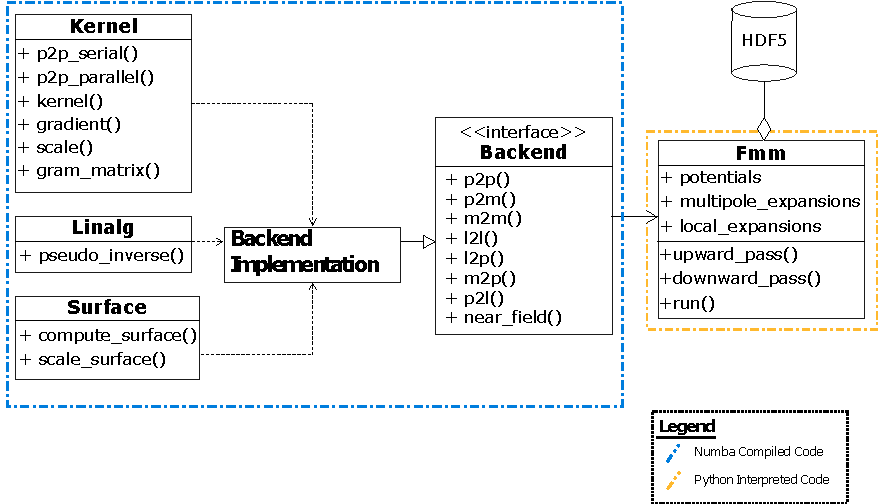
\includegraphics {ch_4/software.pdf}}
    \caption{Simplified UML model of all PyExaFMM components. Trees and other precomputed quantities are stored in a HDF5 database. The `Fmm' object acts as the user interface, all other components are modules consisting of methods operating on arrays, adapted from \cite{kailasa2022pyexafmm}.}
    \label{fig:sec_2_2:design}
\end{figure}

\subsection*{Multithreading in Numba}

Numba enables multithreading via a simple parallel for loop syntax (see listing (\ref{code:sec_2_2:parallel_multithreading})) reminiscent of OpenMP. Internally Numba can use either OpenMP or Intel TBB to generate multithreaded code. We choose OpenMP for PyExaFMM, as it's more suited to functions in which each thread has an approximately similar workload. The threading library can be set via the \lstinline{NUMBA_THREADING_LAYER} environment variable.

Numerical libraries such as NumPy and SciPy implement many of their mathematical operations using multithreaded compiled libraries internally, such as OpenBLAS or IntelMKL. Numba compiled versions of these operations retains this internal multithreading. This leads to \textit{nested parallelism} when combined with a multithreaded region declared with Numba, as in listing (\ref{code:sec_2_2:parallel_multithreading}). This is where a parallel region calls a function with another parallel region inside it. Threads created by the two functions are not coordinated by Numba, and this leads to \textit{oversubscription}, where the number of active threads exceeds the CPU's hardware capacity. Many threads are left idle while the CPU is forced to jump between threads operating on different data. This leads to broken cache locality, and hanging threads threads, stuck waiting for others to finish \cite{malakhov2016python}. We avoid this in PyExaFMM by explicitly setting NumPy operations to be single threaded, via the environment variable \lstinline{OMP_NUM_THREADS=1}, before starting our program. This ensures that the only threads created are those explicitly declared using Numba.


\subsection*{Parallising PyExaFMM}

The $T^{P2M}$, $T^{P2L}$, $T^{M2P}$ and $T^{L2P}$ all rely on the $P2P$ operator, as this computes (\ref{eq:ch_2:two_box_calc}) over their respective sources and targets, and are parallelized over their targets the leaf nodes. For the $T^{L2P}$ operator we encourage cache locality for the $P2P$ step, and keep the data structures passed to Numba as simple as possible, by allocating 1D vectors for the source positions, target positions and the source expansion coefficients, such that all the data required to apply an operator to single target node is adjacent in memory. By storing a vector of `index pointers', that bookend the data corresponding to each target in these 1D vectors, we can form parallel for loops over each target to compute the $P2P$ that encourages cache-locality in the CPU. In order to to this, we have to first iterate through the target nodes, and lookup the associated data to fill the cache local vectors.

The speedup achieved with this strategy, in comparison to a naive parallel iteration over the $T^{L2P}$'s targets, increases with the number of calculations in each thread and hence the expansion order $p$. In an experiment with 32768 leaves, the maximum number of points per leaf, $n_{crit} = 150$, and expansion order $P=10$, our strategy is $13$ \% faster. This corresponds to a realistic FMM problem with approximately $1e6$ randomly distributed particles.

Due to their large interaction lists, the previous strategy is too expensive in terms of memory for the near field, $T^{M2L}$ and $T^{M2P}$ operators. For example, allocating an array large enough to store the maximum possible number of source particle coordinates in double precision for the $T^{M2P}$ operator; with $|W|=148$ and $n_{crit}=150$, requires $\sim 17$GB, and a runtime cost for memory allocations that exceeds the computation time. Instead, for the $T^{M2L}$ we perform a parallel loop over the target nodes at each given level, and over the leaf nodes for the M2P and near field, looking up the relevant data from the linear tree as needed. The $T^{P2L}$ interaction list of each target is at most 19 nodes, and the P2M must also calculate a check potential, cancelling out any speedup from cache locality for these operators.

The matrices involved in the $T^{M2M}$ and $T^{L2L}$ operators can be precomputed and scaled at each level \cite{wang2021exafmm}, and their application is parallelized over all nodes at a given level. Multithreading in this way means that we call the P2P, $T^{P2M}$, $T^{M2P}$, $T^{L2P}$ and near field operators once during the algorithm, the $T^{M2L}$ and $T^{L2L}$ are called $d-2$ times, and the $T^{M2M}$ is called $d$ times, where $d$ is the depth of the octree. This is the minimum number of calls while keeping the operator implementations separate for unit testing.

Figure (\ref{fig:sec_2_2:cpu_wall}) compares the time spent within each Numba-compiled operator (`CPU time') to the total runtime (`wall time') of each operator. The results are computed over five trials over $32768$ leaves, with $n_{crit}=150$ and $P=6$, for a random distribution of $1e6$ charges distributed on the surface of a sphere representing a typical FMM problem. The mean size of the interaction lists are $|U|=11$, $|V|=42$, $|X|=3$, $|W|=3$, and the entire algorithm is computed in $5.95 \pm 0.02 s$, with an additional $9.00 \pm 0.01 s$ for operator pre-computations for a given dataset, which is unachievable in ordinary single-threaded interpreted Python.

The wall time includes the time to (un)box data, organize inputs for Numba compiled functions, and pass control between Numba and Python. Except for the $T^{L2P}$ which has a different parallelization strategy that requires significant data organization that must take place within the GIL restricted Python interpreter, the runtime costs are less than 5 \% of each operator's total wall time, implying that we are nearly always running multithreaded code and utilizing all available CPU cores. 

 \begin{figure}
	\centerline{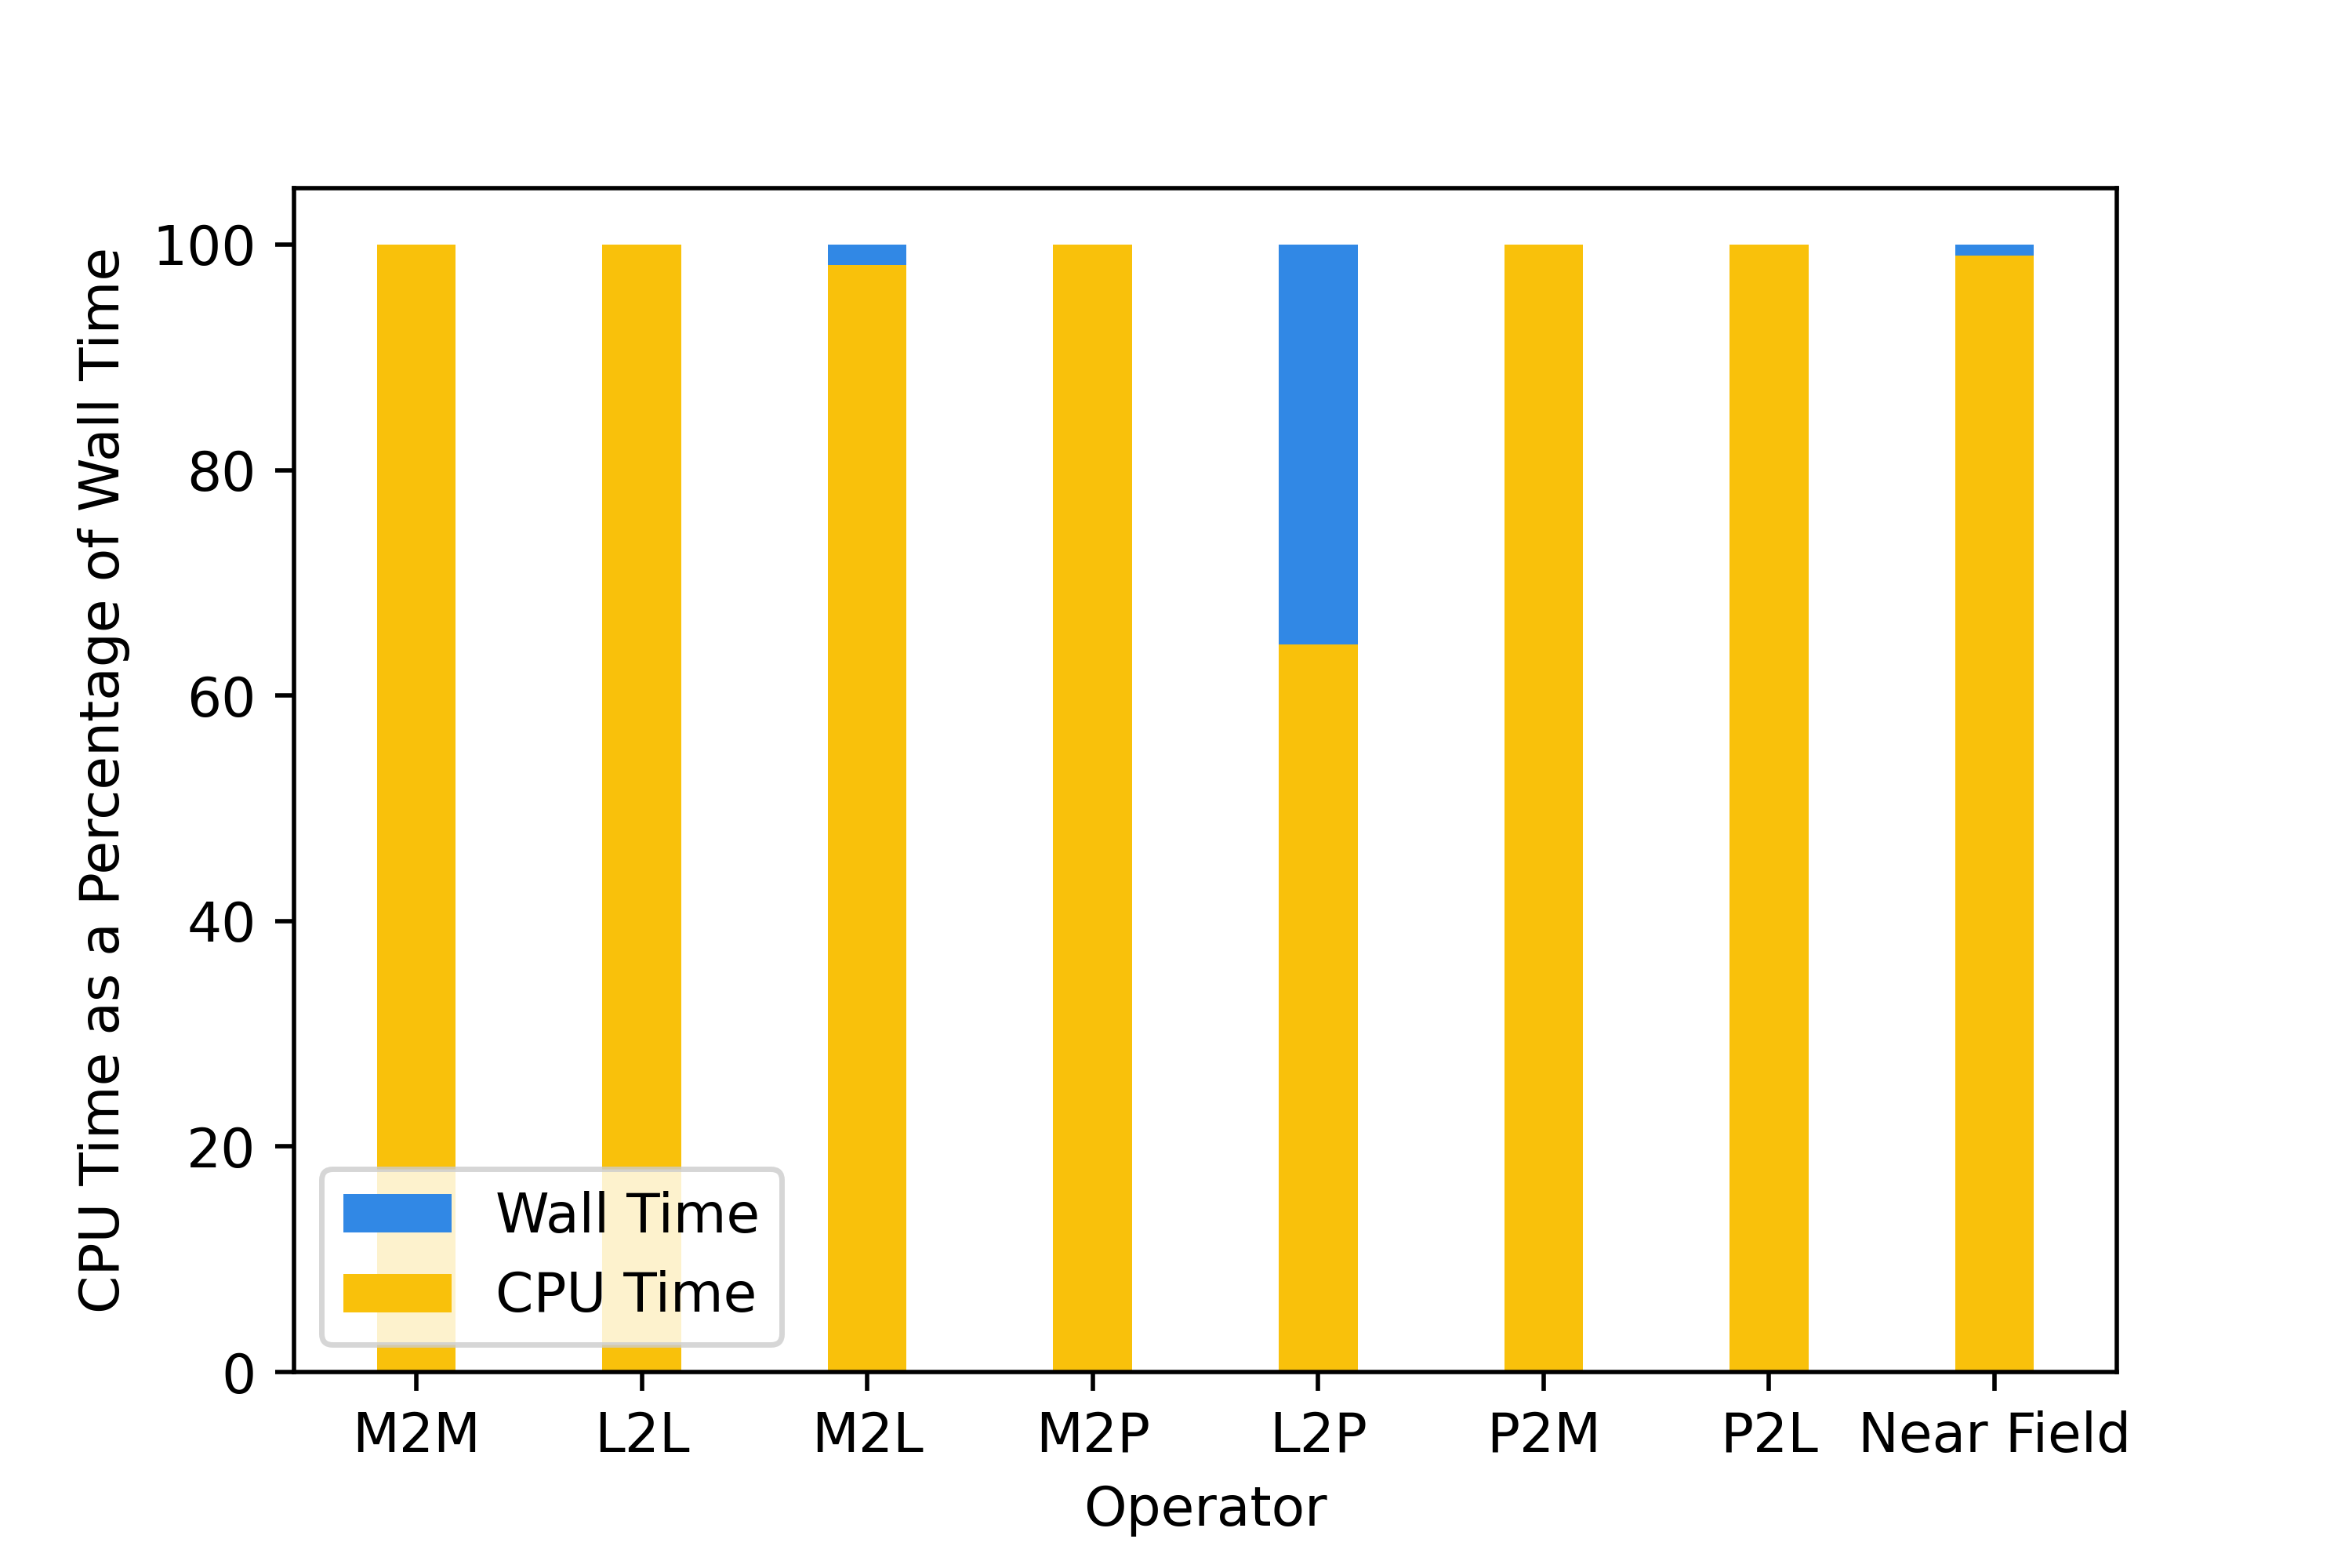
\includegraphics[width=8cm]{ch_4/cpu_wall.png}}
    \caption{CPU time as a percentage of wall time for operators. CPU time is defined as the time in which the algorithm runs pure Numba compiled functions. Wall time is CPU time in addition to the time taken to return control to the Python interpreter, adapted from \cite{kailasa2022pyexafmm}. } 
	\label{fig:sec_2_2:cpu_wall}
\end{figure}


\subsection*{Conclusion}

Achieving optimal multithreaded performance with Numba requires careful consideration of the algorithm being accelerated, details of Numba's backend implementation, as well as a design that suits Numba's data oriented framework. The pitfalls illustrated above show how a user must potentially adapt their code significantly in order to achieve the best performance. Altogether, Numba accelerated code may look decidedly un-Pythonic despite using Python syntax. The complexities involved when using Numba to implement a non-trivial algorithm contrast with its advertisement as a simple way of injecting performance into Python code by applying a decorator. Significant software development expertise is needed in order to optimise a Numba implementation, and arguably more than many in its intended target audience can be expected to possess. 

Despite this, Numba is a remarkable tool. Projects which value Python's expressiveness, simple cross platform builds, as well as large open source ecosystem, and only contain a small number of isolated performance bottlenecks would benefit the most from a Numba implementation. Indeed, by writing only in Python our project size is kept minimal with the entire project running to just 4901 lines of code. Furthermore, we are able to deploy PyExaFMM cross platform trivially with Conda and distribute our software in popular Python channels. 

Resultantly, we wish to find a middle way, that would retain the usability of a higher level language, with the performance benefits of writing in a lower level language, filling the gap from the handoff between a high-level language interface and the programming constraints, as well as the handoff performance hit of a JIT. We believe that this is offered by Rust, which despite being a compiled language, that retains many of these features. 

\begin{figure}
    \centerline{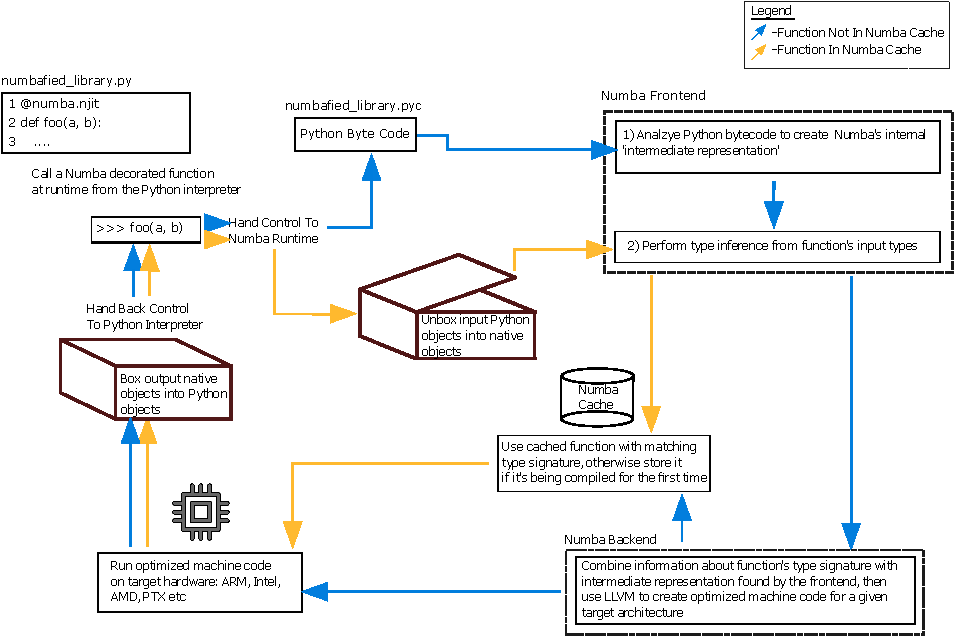
\includegraphics{ch_4/numba.pdf}}
    \caption{Simplified execution path when calling a Numba compiled function from the Python interpreter. The blue path is only taken if the function hasn't been called before. The orange path is taken if a compiled version with the correct type signature already exists in the Numba cache, adapted from \cite{kailasa2022pyexafmm}.}
    \label{fig:sec_2_2:numba_runtime}
\end{figure}

\pythonexternal[basicstyle=\footnotesize, caption={An example of parallel multithreading.}\label{code:sec_2_2:parallel_multithreading}]{snippets/parallel_multithreading.py}
\pythonexternal[basicstyle=\footnotesize, caption={An example of using Numba in a Python function operating on ndarrays.}\label{code:sec_2_2:loop_fusion}]{snippets/loop_fusion.py}

\pythonexternal[basicstyle=\footnotesize,caption={Three ways of writing a trivial algorithm that passes around a vector, while performing some computations.}\label{code:sec_2_2:nested_function}]{snippets/nested_function.py}